\documentclass[aspectratio=169,11pt]{beamer}
\usetheme{default}
\useinnertheme{circles}
\setbeamertemplate{navigation symbols}{}
\setbeamertemplate{footline}[frame number]
\usepackage{amsmath,amssymb,bm,booktabs,graphicx}
\definecolor{miptblue}{RGB}{0,84,166}
\setbeamercolor{title}{fg=miptblue}
\setbeamercolor{frametitle}{fg=miptblue,bg=white}
\setbeamercolor{itemize item}{fg=miptblue}
\setbeamercolor{enumerate item}{fg=miptblue}
\setbeamerfont{frametitle}{series=\bfseries}
\newcommand{\norm}[1]{\left\|#1\right\|}
\newcommand{\MSA}{\operatorname{MSA}}
\newcommand{\FFN}{\operatorname{FFN}}
\newcommand{\TB}{\operatorname{TB}}
\newcommand{\diag}{\operatorname{diag}}
\title{Jacobian Analysis of a Recurrent\texorpdfstring{\\}{ }Transformer Block}
\author{Dmitrii Vasilenko\inst{1} \and Ilia Stepanov\inst{1} \and Vadim Kasiuk\inst{1}\texorpdfstring{\\}{, }
Gleb Karpeev\inst{1} \and Andrey Grabovoy\inst{1,2}}
\institute{\inst{1}Moscow Institute of Physics and Technology\\
\inst{2}V.A. Trapeznikov Institute of Control Sciences\\
of Russian Academy of Sciences}
\date{AINL 2026\\\small Revised November 2, 2026}

\begin{document}
\begin{frame}[plain]
\titlepage
\end{frame}

\begin{frame}{A recurrent block is a discrete dynamical system}
\[
Y^{(t+1)}=F_\nu(Y^{(t)}),\qquad Y^{(t)}\in\mathbb{R}^{S\times D}.
\]
\begin{itemize}
\item The same block parameters are reused at every iteration.
\item The one-step Jacobian measures how an input perturbation changes after
one update.
\item We bound this Jacobian for a block containing attention, an FFN,
residual connections, and RMSNorm.
\end{itemize}
\vspace{1em}
\small
Tomihari and Karakida (2025) give the corresponding normalization argument
for recurrent self-attention. Here it is composed through both sub-blocks.
\end{frame}

\begin{frame}{The update under study}
\begin{align*}
Z_1&=Y+\MSA(Y), &Y'&=R_1(Z_1),\\
Z_2&=Y'+\FFN(Y'), &\TB(Y)&=R_2(Z_2),\\
\Delta(Y)&=C+\TB(Y), &U_\nu&=Y+\nu\Delta(Y),\\
&&F_\nu(Y)&=R_U(U_\nu).
\end{align*}
\begin{itemize}
\item $R_1,R_2,R_U$ are separate, row-wise normalization layers.
\item The context $C$ is fixed during each trajectory and when computing
$J_{F_\nu}(Y)$.
\item In the trajectory experiment, $C=0.1Y^{(0)}$.
\end{itemize}
\end{frame}

\begin{frame}{RMSNorm: convention and derivative}
For a token $y\in\mathbb{R}^D$ and layer $\ell\in\{1,2,U\}$,
\[
\rho_\ell(y)=\sqrt{\norm{y}_2^2/D+\epsilon_\ell},\qquad
R_\ell(y)=\diag(\gamma_\ell)\frac{y}{\rho_\ell(y)},\quad
\epsilon_\ell>0.
\]
\[
J_{R_\ell}(y)=\frac{\diag(\gamma_\ell)}{\rho_\ell(y)}
\left(I-\frac{yy^\top}{D\rho_\ell(y)^2}\right),\qquad
\norm{J_{R_\ell}(y)}_2\leq\frac{g_\ell}{\rho_\ell(y)},
\]
where $g_\ell=\norm{\gamma_\ell}_\infty$.
\vspace{0.5em}
\begin{itemize}
\item The factor decreases as the normalization input grows.
\item It can exceed one when the input denominator is small.
\item With $\epsilon_\ell>0$, the matrix in parentheses is not an exact projector.
\end{itemize}
\end{frame}

\begin{frame}{Theorem 3.1: one-step Jacobian bound}
Use the smallest denominator across tokens at each layer:
\[
r_1=\min_i\rho_1((Z_1)_i),\quad
r_2=\min_i\rho_2((Z_2)_i),\quad
r_U=\min_i\rho_U((U_\nu)_i).
\]
Let $M=\norm{J_{\MSA}(Y)}_2$ and $L=\norm{J_{\FFN}(Y')}_2$. Then
\[
\boxed{\norm{J_{F_\nu}(Y)}_2\leq
\frac{g_U}{r_U}\left[1+\nu\frac{g_2g_1}{r_2r_1}(1+L)(1+M)\right].}
\]
\vspace{1em}
\begin{itemize}
\item This follows from the chain rule and submultiplicativity.
\item Component norms are evaluated at their actual inputs.
\item An average token denominator cannot replace the minimum.
\end{itemize}
\end{frame}

\begin{frame}{Theorem 3.2: boundedness as the step grows}
Fix $Y$, $C$, all weights, and all normalization parameters. Suppose
\[
\delta=\min_i\norm{\Delta(Y)_i}_2>0.
\]
Let $B=\max_i\norm{Y_i}_2$ and
$K=g_2g_1(1+L)(1+M)/(r_2r_1)$. For $\nu\geq2B/\delta$,
\[
r_U\geq\frac{\nu\delta}{2\sqrt D},\qquad
\norm{J_{F_\nu}(Y)}_2\leq
\frac{2\sqrt D\,g_U}{\delta}\left(K+\frac1\nu\right)=O(1).
\]
\vspace{1em}
The outer denominator grows with $\nu$ and compensates for the step multiplier.
The result is pointwise in the fixed state and parameters.
\end{frame}

\begin{frame}{Bounded in step size does not mean convergent in time}
For fixed context, derivatives through a trajectory involve a product:
\[
\frac{\partial Y^{(T)}}{\partial Y^{(0)}}
=J_{F_\nu}(Y^{(T-1)})\cdots J_{F_\nu}(Y^{(0)}).
\]
\begin{itemize}
\item A constant one-step bound $k>1$ allows the product bound $k^T$.
\item Local asymptotic stability of a fixed point follows from spectral radius
less than one; a norm below one is a stronger sufficient condition.
\item A large one-step singular value alone does not prove chaos or exponential
growth along a trajectory.
\end{itemize}
\vspace{0.5em}
For example, $x\mapsto-x$ on a sphere has bounded derivative and period-two
orbits. This illustrates why a bounded norm is insufficient.
\end{frame}

\begin{frame}{Experimental protocol}
All blocks and image projections are untrained. Normalization scales start at
one and $\epsilon=10^{-8}$.
\vspace{1em}
\begin{center}
\begin{tabular}{lcccc}
\toprule
Experiment & $S$ & $D$ & $H$ & $D_{\rm ff}$\\
\midrule
One-step bound & 16 & 32 & 4 & 64\\
Large-step sweep & 16 & 32 & 4 & 64\\
Trajectories & 32 & 64 & 4 & 128\\
\bottomrule
\end{tabular}
\end{center}
\begin{itemize}
\item Experiments 1 and 2: dense autograd Jacobians and SVD, float64.
\item Weights, state, and context are fixed within each step-size sweep.
\item Trajectories: 1000 steps, $\nu\in\{0.1,0.5,1.0\}$;
25 trials per dataset and step size.
\end{itemize}
\end{frame}

\begin{frame}{Experiment 1: check the composed bound}
\begin{center}
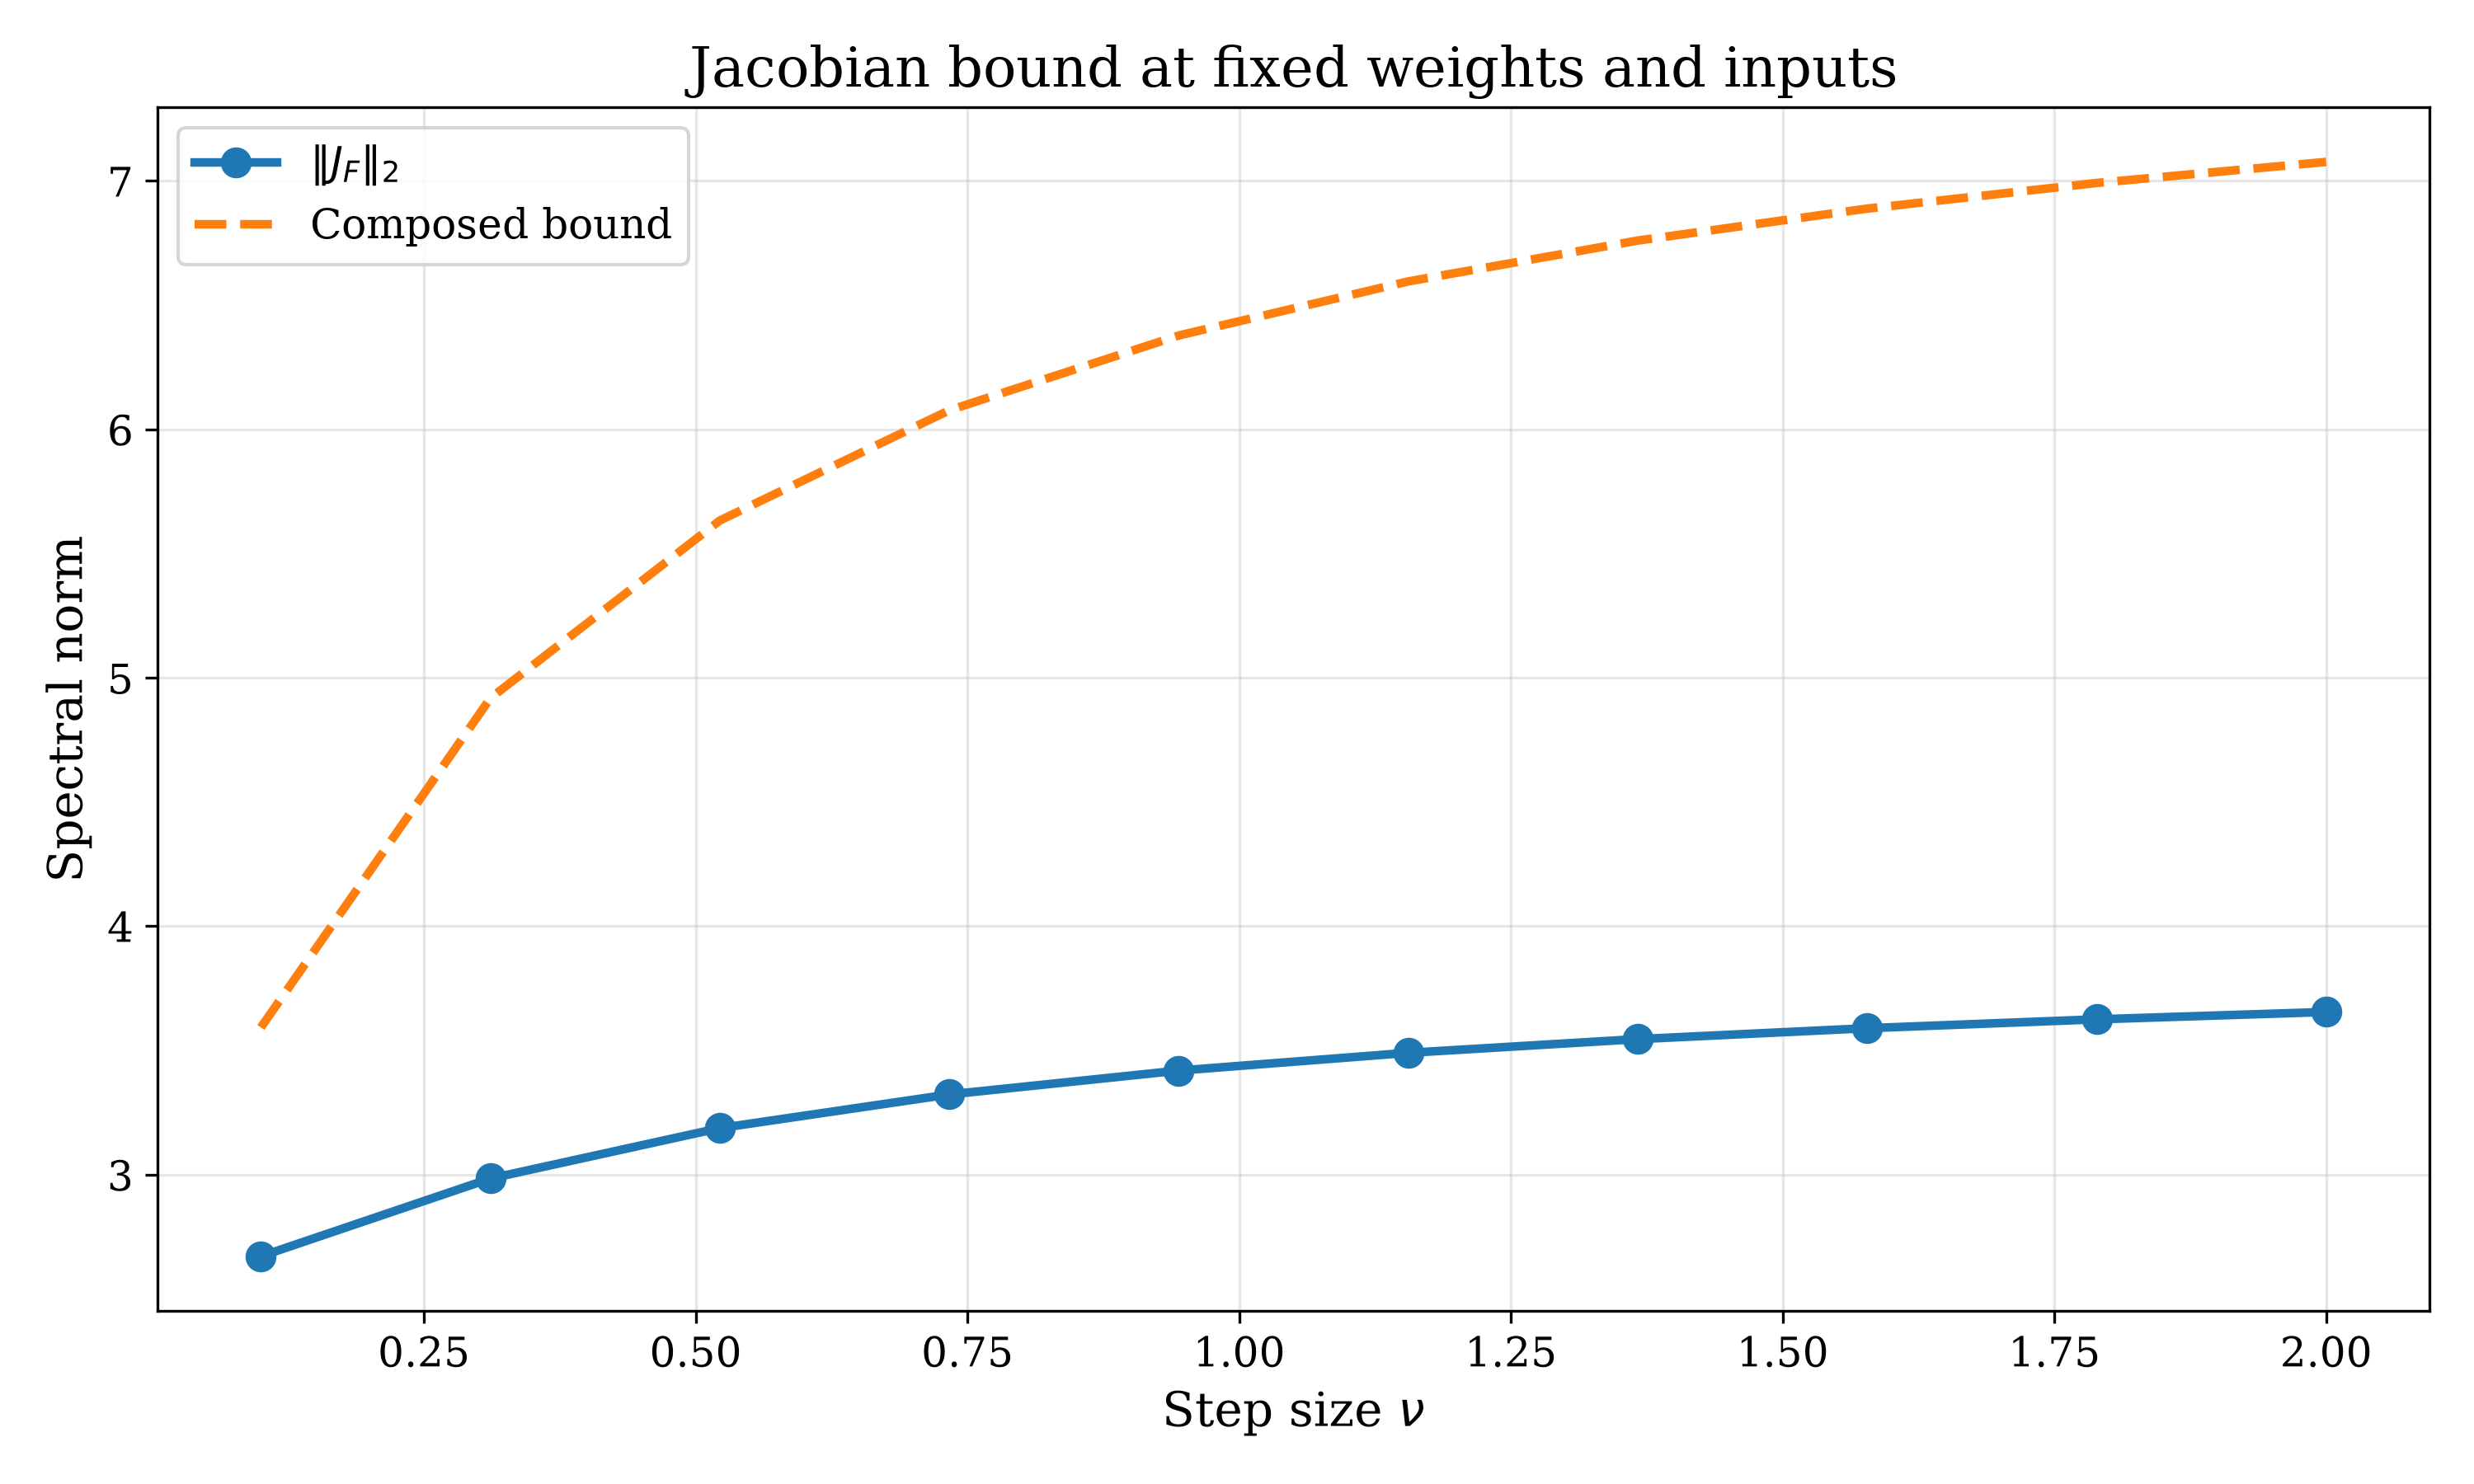
\includegraphics[width=0.72\textwidth,height=0.69\textheight,keepaspectratio]{../plots/fig1_bounds_validation.png}
\end{center}
\small
Seed 42; ten step sizes in $[0.1,2.0]$. Both component Jacobian norms and all
three token minima enter the bound.
\end{frame}

\begin{frame}{Experiment 2: compare fixed-model sweeps}
\begin{center}
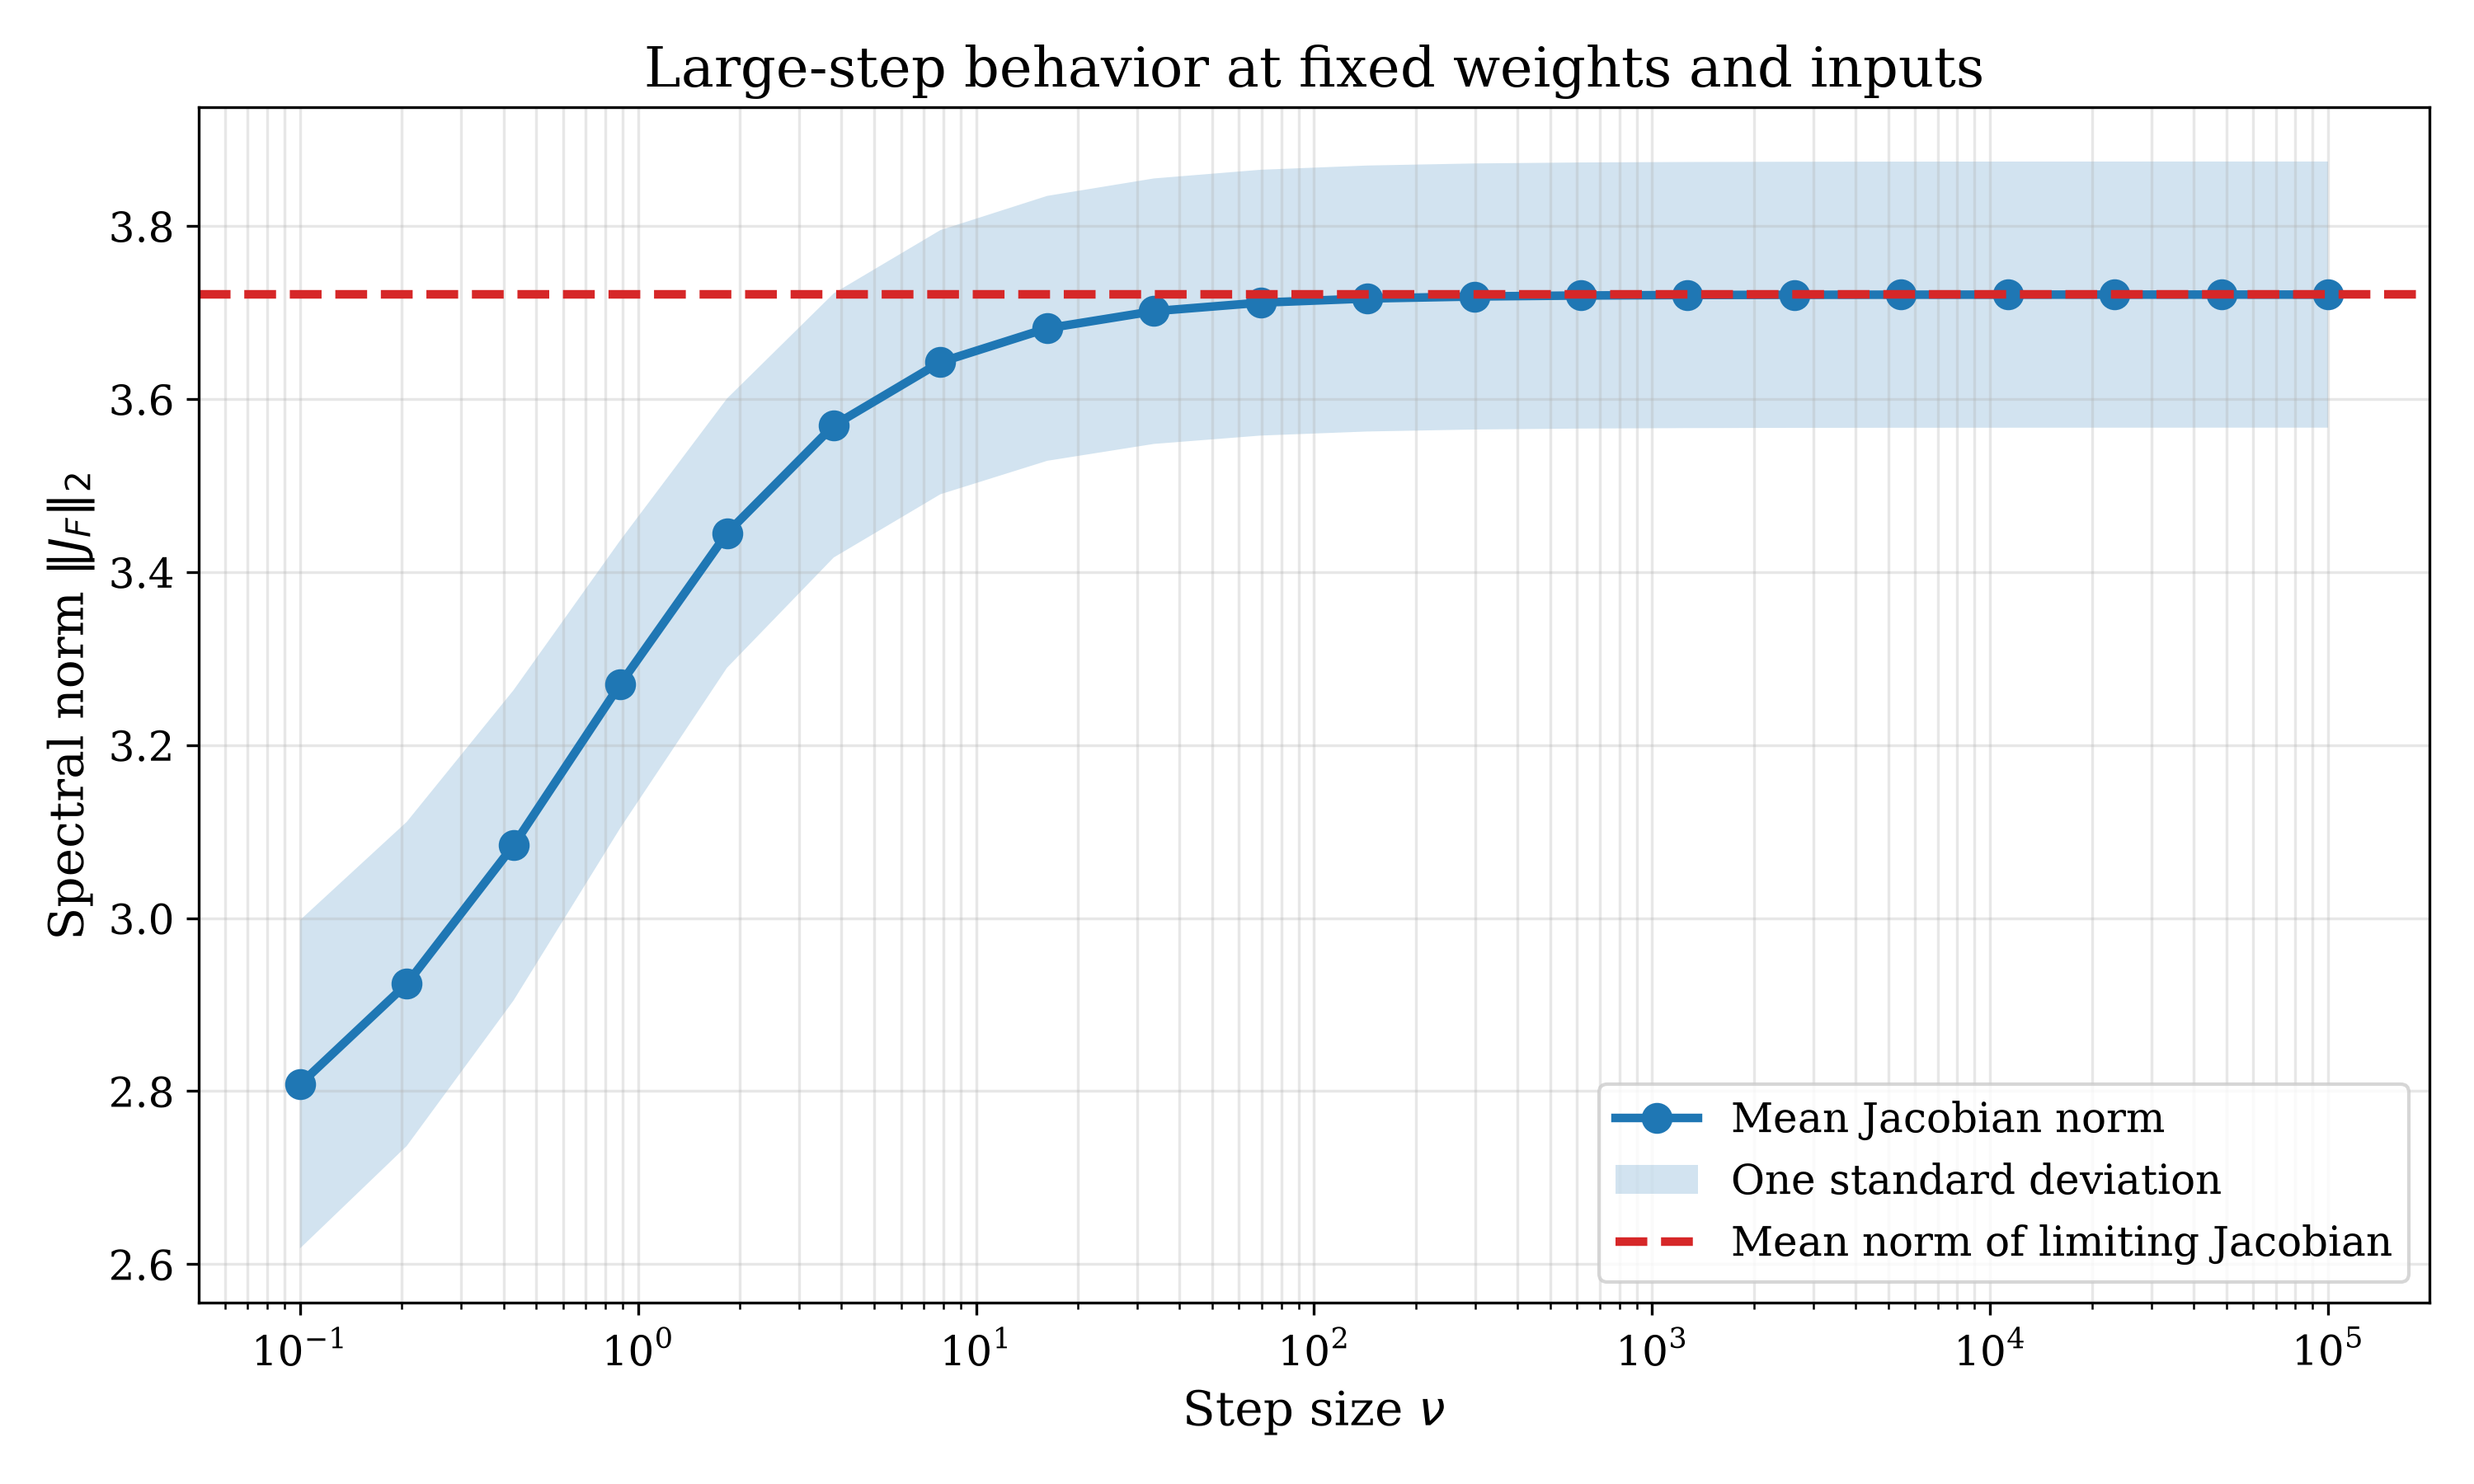
\includegraphics[width=0.72\textwidth,height=0.69\textheight,keepaspectratio]{../plots/fig2_asymptotic.png}
\end{center}
\small
Twenty step sizes from $10^{-1}$ to $10^5$; seeds 0--9. Shading is one
standard deviation across seeds. At $\nu=10^5$, the mean norm is $3.720649$;
the independently computed limiting mean is $3.720655$.
\end{frame}

\begin{frame}{Experiment 3: measure successive-state differences}
\begin{center}
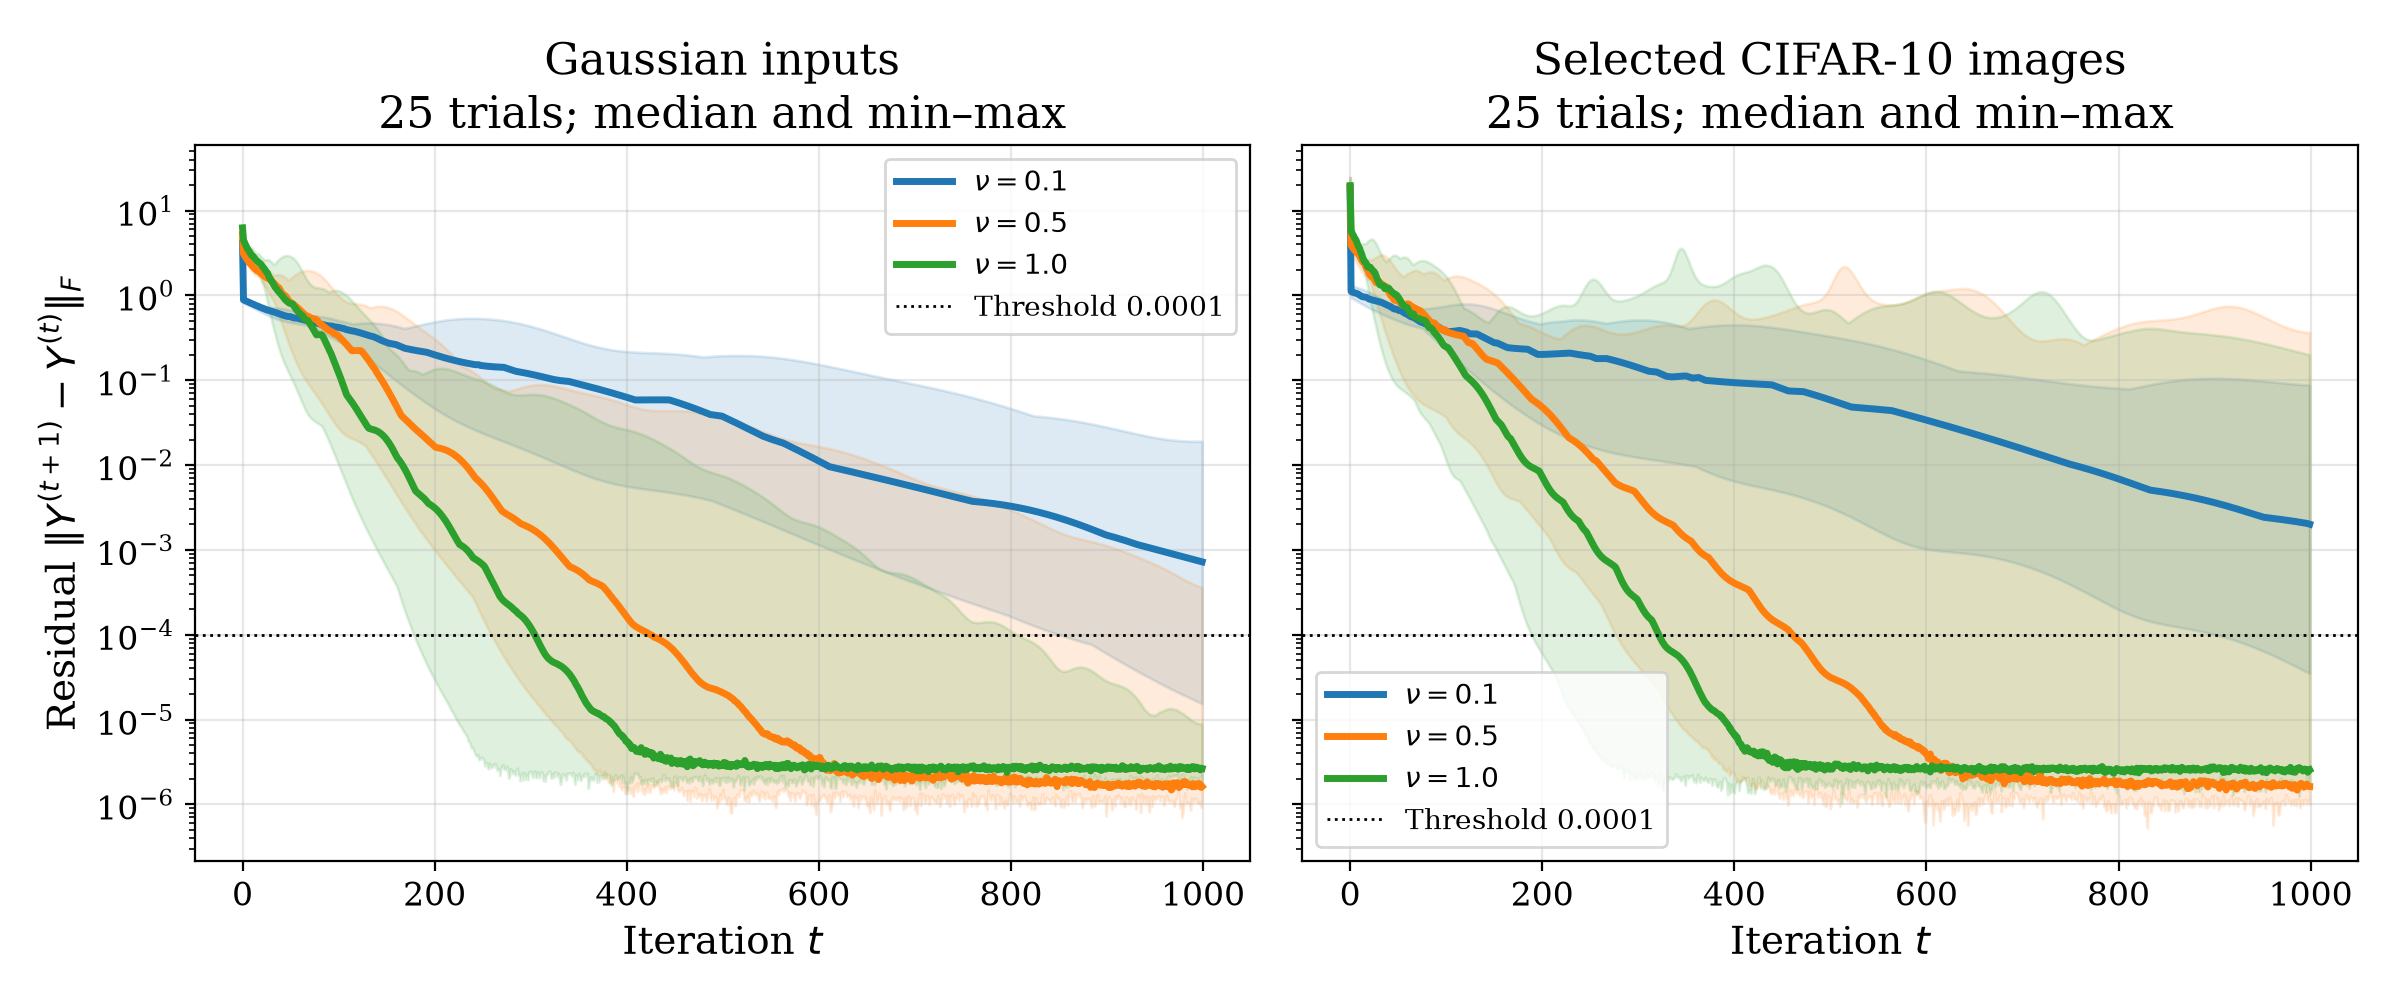
\includegraphics[width=0.94\textwidth,height=0.68\textheight,keepaspectratio]{../plots/fig3_contraction.png}
\end{center}
\small
Seeds 0--4; five Gaussian inputs and CIFAR-10 test images 0--4 per seed.
Curves show medians; bands span the observed minimum and maximum.
\end{frame}

\begin{frame}{Interpreting the trajectory experiment}
The criterion is $d_t=\norm{Y^{(t+1)}-Y^{(t)}}_F\leq10^{-4}$
throughout the final 20 of 1000 steps.
\begin{center}
\begin{tabular}{lccc}
\toprule
Input & $\nu=0.1$ & $\nu=0.5$ & $\nu=1.0$\\
\midrule
Gaussian & 6/25 & 23/25 & 25/25\\
CIFAR-10 & 6/25 & 20/25 & 22/25\\
\bottomrule
\end{tabular}
\end{center}
\begin{itemize}
\item The counts increase with $\nu$ in this sample; this is not a general guarantee.
\item Missing the threshold by step 1000 does not prove non-convergence.
\item The residual measures progress toward a fixed point on one trajectory,
not contraction between different initial states.
\end{itemize}
\end{frame}

\begin{frame}{What the analysis establishes}
\begin{itemize}
\item An explicit bound for the one-step Jacobian of the complete update.
\item Separate contributions from attention, FFN, and each normalization layer.
\item A bounded large-step limit at fixed state and parameters when every
update row is nonzero.
\end{itemize}
\vspace{1em}
Contraction and gradient control over many recurrent steps require additional
conditions. They are not consequences of the large-step bound alone.
\end{frame}

\begin{frame}{References and materials}
\small
A.~Tomihari and R.~Karakida (2025).
\emph{Recurrent Self-Attention Dynamics: An Energy-Agnostic Perspective from
Jacobians}. arXiv:2505.19458v3. Proposition 5.1 and Lemma A.3.
\vspace{1em}

B.~Zhang and R.~Sennrich (2019).
\emph{Root Mean Square Layer Normalization}. NeurIPS 32.
\vspace{1.5em}

\href{https://github.com/Dimundel/Jacobian-Analysis-of-a-Recurrent-Transformer-Block}{Code, revised manuscript, and numerical records}
\vspace{1em}

\texttt{vasilenko.dmitrii@phystech.edu}
\end{frame}
\end{document}
